\documentclass[10pt,compress,aspectratio=169]{beamer}
%Information to be included in the title page:
\title{Title of the Presentation}
\newcommand{\footertitle}[1]{\def\insertfootertitle{#1}}
\footertitle{Short Title}
\author{Austin Widmer}
\institute{Texas A\& University: Department of Aerospace Engineering}
\date{\today} 
\usepackage{amsmath}
\usepackage{caption}
\usepackage{graphicx,comment}
\usepackage[english]{babel}
\usepackage{graphicx}
\usepackage{rotating}
\usepackage{multicol}
\usepackage{hyperref}
\usepackage{enumerate}
\usepackage{tikz}
\usepackage{graphicx}
\usepackage{bm}
\usepackage[T1]{fontenc}
\usepackage[scaled=0.95]{helvet}
\renewcommand{\familydefault}{\sfdefault}
\usepackage{xcolor}

\definecolor{tamu_maroon}{HTML}{500000}
\definecolor{tamu_white}{HTML}{FFFFFF}
\definecolor{tamu_black}{HTML}{202020}
\definecolor{tamu_dark_gray}{HTML}{3E3E3E}
\definecolor{tamu_gray}{HTML}{707070}
\definecolor{tamu_light_gray}{HTML}{D1D1D1}
\definecolor{tamu_tan}{HTML}{D6D3C4}
\definecolor{tamu_dark_maroon}{HTML}{3C0000}
\definecolor{tamu_light_maroon}{HTML}{732F2f}
 

\setbeamercolor{structure}{fg=tamu_maroon}
\setbeamercolor{frametitle}{fg=tamu_maroon}

%%%%%%%%%%%%%%%%%%%%%%%%%%%%%%%%%%%%%%%%%%%%%%%%%%%%%%%%%%%%%%%%%%%%%%%%%%%%%%%%%%%%%%%%%%%%%%%%%%%%%%%%%%%%%%

\setbeamertemplate{title page}{
	\begin{tikzpicture}[remember picture,overlay]
        % PNG positioned from the top-left corner
        \node[anchor=north] at
            ([yshift=-0.1cm]current page.north) {
                
\includegraphics[width=4.5cm]{logos/tamu_engineering.png}
            };
        % Title box
        \node[
            fill=tamu_white,
            fill opacity=0.92, 
            text opacity=1, 
            text width=0.75\paperwidth,
            align=center,
            inner sep=14pt
        ] at ([yshift=-2cm]current page.center) {
			{\usebeamerfont{title}\usebeamercolor[fg]{title}\bfseries\inserttitle\par}
			\vspace{0.10cm}
			{\usebeamerfont{author}\usebeamercolor[fg]{author}\bfseries\insertauthor\par}
			% {\usebeamerfont{institute}\usebeamercolor[fg]{institute}\insertinstitute\par}
			{\usebeamerfont{date}\usebeamercolor[fg]{date}\bfseries\insertdate\par}
		};
	\end{tikzpicture}
}

\makeatletter

\setbeamercolor{frametitle}{fg=tamu_white,bg=tamu_black}
\setbeamercolor{footline}{fg=tamu_white,bg=tamu_black}

\defbeamertemplate*{frametitle}{basic}{%
    \nointerlineskip%
    \begin{beamercolorbox}[
        wd=\paperwidth,
        ht=1.05cm,
        dp=0.25cm,
        leftskip=0.35cm,
        rightskip=0.35cm
    ]{frametitle}%
        \usebeamerfont{frametitle}\insertframetitle%
        \hfill
        \raisebox{-0.18cm}[0pt][0pt]{%
            \begin{tabular}[b]{@{}r@{}}
                {\tiny\color{tamu_white}\insertauthor\,|\,\insertdate}\\[2pt]
                
\includegraphics[height=0.72cm]{logos/tamu_engineering.png}
            \end{tabular}%
        }%
    \end{beamercolorbox}%
}

\setbeamertemplate{frametitle}[basic]

% Per-frame section data is written to the .aux and read back on the next compile.
\newcount\fp@C
\newcount\fp@idx
\def\fp@rec#1#2#3{\global\@namedef{fp@sec@#1}{#2}\global\@namedef{fp@name@#2}{#3}}
\def\fp@sec#1{\ifcsname fp@sec@#1\endcsname\csname fp@sec@#1\endcsname\else0\fi}
\def\fp@record{\protected@write\@auxout{}{\string\fp@rec{\the\c@framenumber}{\the\c@section}{\insertsection}}}
\def\fp@recordexcluded{\protected@write\@auxout{}{\string\fp@rec{\the\c@framenumber}{0}{\insertsection}}}
\def\fp@gap{8.5}

\def\fp@progress{%
    \edef\fp@S{\number\beamer@sectionmax}%
    \edef\fp@T{\number\inserttotalframenumber}%
    \ifnum\fp@S>0 \ifnum\fp@T>0
        \global\fp@C=0
        \foreach \fps in {1,...,\fp@S}{\global\@namedef{fp@n@\fps}{0}}%
        \foreach \fpf in {1,...,\fp@T}{%
            \edef\fp@s{\fp@sec{\fpf}}%
            \ifnum\fp@s>0
                \ifnum\fp@s>\fp@S\else
                    \global\advance\fp@C by 1
                    \ifnum\csname fp@n@\fp@s\endcsname=0
                        \global\expandafter\edef\csname fp@first@\fp@s\endcsname{\the\fp@C}%
                    \fi
                    \global\expandafter\edef\csname fp@n@\fp@s\endcsname{\the\numexpr\csname fp@n@\fp@s\endcsname+1\relax}%
                \fi
            \fi
        }%
        \ifnum\fp@C>0
            \pgfmathsetmacro\fp@p{(\paperwidth-0.7cm-\fp@S*\fp@gap pt-5pt)/\number\fp@C}%
            \pgfmathsetmacro\fp@r{min(0.09cm,0.4*\fp@p)}%
            \global\fp@idx=0
            \makebox[\dimexpr\paperwidth-0.7cm\relax][c]{%
            \begin{tikzpicture}[x=1pt,y=1pt,baseline=0pt]
                \foreach \fpf in {1,...,\fp@T}{%
                    \edef\fp@s{\fp@sec{\fpf}}%
                    \ifnum\fp@s>0
                        \ifnum\fp@s>\fp@S\else
                            \global\advance\fp@idx by 1
                            \pgfmathsetmacro\fp@x{(\number\fp@idx-0.5)*\fp@p+(\fp@s-1)*\fp@gap}%
                            \ifnum\fpf>\insertframenumber
                                \draw[tamu_white,line width=0.6pt] (\fp@x,0) circle (\fp@r pt);
                            \else
                                \fill[tamu_white] (\fp@x,0) circle (\fp@r pt);
                            \fi
                        \fi
                    \fi
                }
                \foreach \fps in {1,...,\fp@S}{%
                    \ifnum\csname fp@n@\fps\endcsname>0
                        \edef\fp@a{\csname fp@first@\fps\endcsname}%
                        \edef\fp@b{\csname fp@n@\fps\endcsname}%
                        \pgfmathsetmacro\fp@lx{((\fp@a-1)+\fp@b/2)*\fp@p+(\fps-1)*\fp@gap}%
                        \pgfmathsetmacro\fp@lw{\fp@b*\fp@p+\fp@gap-2}%
                        \node[anchor=south,text width=\fp@lw pt,align=center,inner sep=0pt,font=\fontsize{4}{4.8}\selectfont,text=tamu_white]
                            at (\fp@lx,7) {\csname fp@name@\fps\endcsname};
                    \fi
                }
            \end{tikzpicture}}%
        \fi
    \fi\fi
}

\setbeamertemplate{footline}{%
    \fp@record
    \begin{beamercolorbox}[
        wd=\paperwidth,
        ht=0.65cm,
        dp=0.16cm,
        leftskip=0.35cm,
        rightskip=0.35cm
    ]{footline}%
        \fp@progress
    \end{beamercolorbox}%
}

\makeatother

% Section title / divider frame.
% Usage: \sectiontitleframe{assets/Earth-1.jpg}{Section Title Text}
\makeatletter
\newcommand{\sectiontitleframe}[2]{%
    \usebackgroundtemplate{\includegraphics[width=\paperwidth,height=\paperheight]{#1}}%
    \begin{frame}[plain]
        \fp@recordexcluded
        \begin{tikzpicture}[remember picture,overlay]
            % Logo box, matching the title page layout
            \node[anchor=north] at
                ([yshift=-0.1cm]current page.north) {
                    
\includegraphics[width=4.5cm]{logos/tamu_engineering.png}
                };
            % Title box
            \node[
                fill=tamu_white,
                fill opacity=0.92,
                text opacity=1,
                text width=0.85\paperwidth,
                align=center,
                inner sep=16pt
            ] at ([yshift=-2.1cm]current page.center) {
                {\usebeamerfont{title}\color{tamu_maroon}\bfseries\LARGE #2\par}
            };
        \end{tikzpicture}
    \end{frame}
    \usebackgroundtemplate{}%
}
\makeatother

\newcommand{\tableofcontentsframe}[1][Contents]{%
    \begin{frame}
        \frametitle{#1}
        \tableofcontents
    \end{frame}
}
%%%%%%%%%%%%%%%%%%%%%%%%%%%%%%%%%%%%%%%%%%%%%%%%%%%%%%%%%%%%%%%%%%%%%%%%%%%%%%%%%%%%%%%%%%%%%%%%%%%%%%%%%%%%%%
  
\begin{document}

{\usebackgroundtemplate{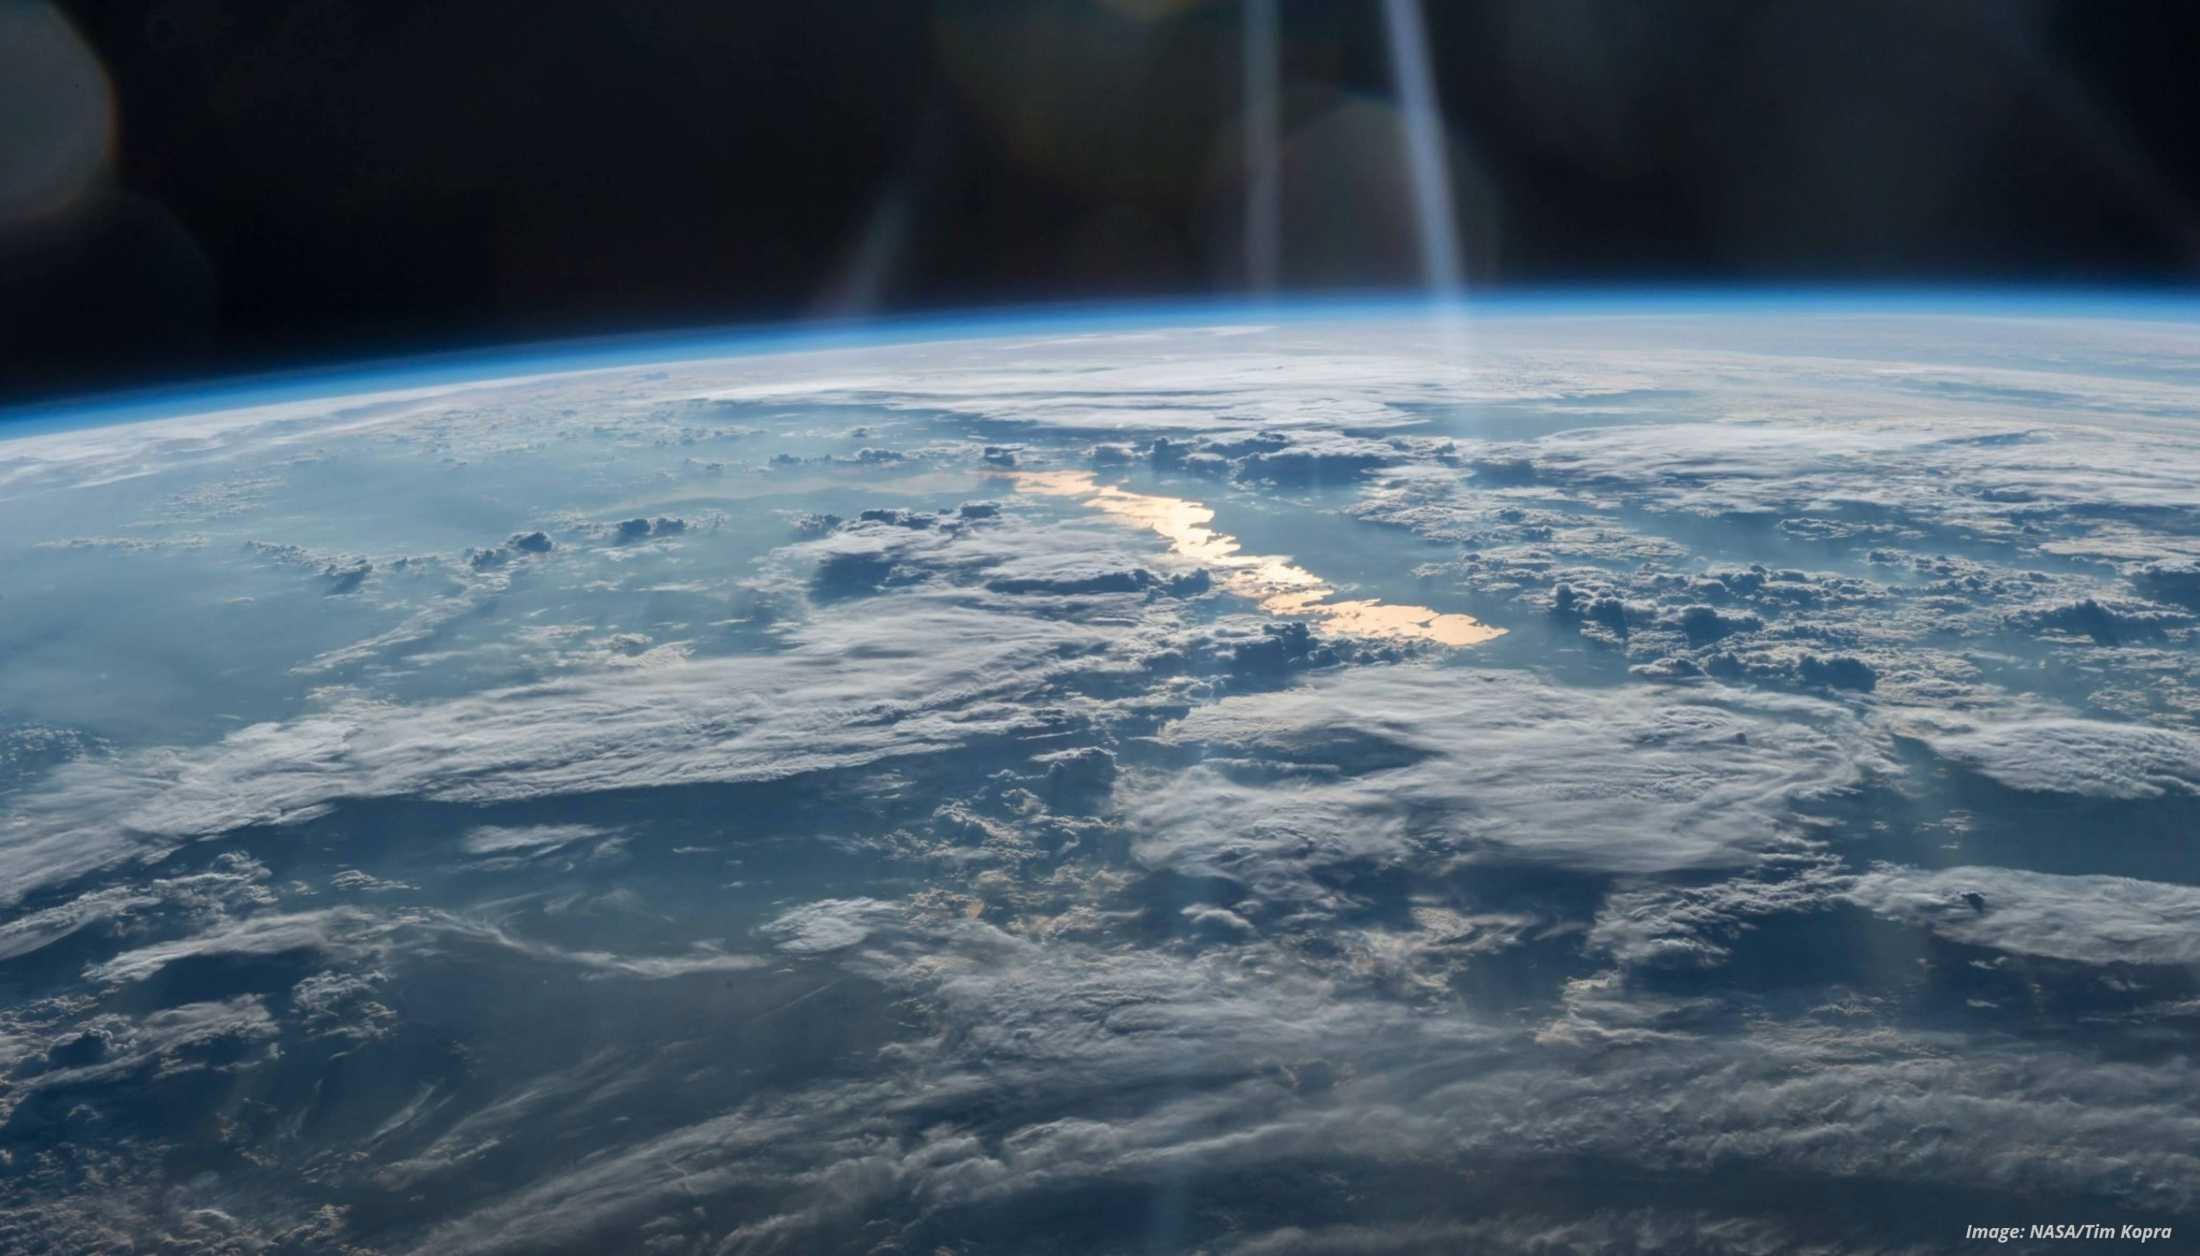
\includegraphics[width=\paperwidth,height=\paperheight]{assets/Earth-1.jpg}}
\frame[plain]{\titlepage}}
% \tableofcontentsframe
% \section{Introduction}

% \begin{frame}
% \frametitle{Sample frame title}
% This is some text in the first frame. This is some text in the first frame. This is some text in the first frame.
% \end{frame}

\section{Slide Format Examples}

% Slide format: compare two approaches with parallel, color-coded blocks.
\begin{frame}
\frametitle{Compare Two Approaches}
Briefly state the question or criterion that makes this comparison useful.
\begin{columns}[T,onlytextwidth]
	\column{0.47\textwidth}
	\begingroup
	\setbeamercolor{block title}{fg=tamu_white,bg=tamu_dark_gray}
	\setbeamercolor{block body}{fg=tamu_black,bg=tamu_light_gray}
	\begin{block}{Approach A}
		\begin{minipage}[t][2.5cm][t]{\linewidth}
		\vspace{0pt}
		\footnotesize
		\begin{itemize}
			\setlength{\itemsep}{0.2em}
			\item Describe the core idea.
			\item Note an important strength.
			\item State a relevant limitation.
		\end{itemize}
		\end{minipage}
	\end{block}
	\endgroup
	\column{0.47\textwidth}
	\begingroup
	\setbeamercolor{block title}{fg=tamu_white,bg=tamu_maroon}
	\setbeamercolor{block body}{fg=tamu_black,bg=tamu_tan}
	\begin{block}{Approach B}
		\begin{minipage}[t][2.5cm][t]{\linewidth}
		\vspace{0pt}
		\footnotesize
		\begin{itemize}
			\setlength{\itemsep}{0.2em}
			\item Describe the core idea.
			\item Note an important strength.
			\item State a relevant limitation.
		\end{itemize}
		\end{minipage}
	\end{block}
	\endgroup
\end{columns}
\end{frame}

% Slide format: pair a concise explanation and equation with a supporting visual.
\begin{frame}
\frametitle{Explain a Model or Process}
State the main idea in one sentence before showing its mathematical or visual detail.
\begin{columns}[T,onlytextwidth]
	\column{0.52\textwidth}
	\small
	Explain the variables or steps needed to interpret the result. Keep the text focused on what the audience should notice.
	\begin{align*}
	\mathrm{Output} &= f(\mathrm{input},\mathrm{parameters}),\\
	\mathrm{change} &= \mathrm{new\ value} - \mathrm{baseline}.
	\end{align*}
	\column{0.45\textwidth}
	\centering
	\fbox{\parbox[c][0.40\textheight][c]{0.91\linewidth}{\centering\small Replace with a schematic,\\plot, or other supporting visual}}
\end{columns}
\vfill
{\tiny Source: Add a concise source note when the slide uses external material.}
\end{frame}

% Slide format: compare a small set of results panels and finish with one takeaway.
\begin{frame}
\frametitle{Compare Results Across Cases}
Summarize the test setup or dataset in one short sentence.
\begin{columns}[T,onlytextwidth]
	\column{0.32\textwidth}
	\centering
	\scriptsize Case A\\[0.3em]
	\fbox{\parbox[c][0.20\textheight][c]{0.90\linewidth}{\centering Replace with plot or image}}
	\column{0.32\textwidth}
	\centering
	\scriptsize Case B\\[0.3em]
	\fbox{\parbox[c][0.20\textheight][c]{0.90\linewidth}{\centering Replace with plot or image}}
	\column{0.32\textwidth}
	\centering
	\scriptsize Error or metric\\[0.3em]
	\fbox{\parbox[c][0.20\textheight][c]{0.90\linewidth}{\centering Replace with plot or image}}
\end{columns}
\vspace{0.4em}
\small
State the main comparison, then support it with one or two concise observations.
\begin{itemize}
	\footnotesize
	\item Report the primary metric with units or a clear definition.
	\item Include a limitation or trade-off when it affects the conclusion.
\end{itemize}
\begingroup
\setbeamercolor{block title}{fg=tamu_white,bg=tamu_dark_gray}
\setbeamercolor{block body}{fg=tamu_black,bg=tamu_light_gray}
\begin{block}{Key takeaway}
\small State the conclusion that the audience should remember.
\end{block}
\endgroup
\end{frame} 

\section{Section Divider Example}
\sectiontitleframe{assets/Moon-1.jpg}{Section Title}

\end{document}

